%$Id: chi06.tex,v 1.4 2006/02/13 23:19:21 rlw Exp rlw $
\documentclass[dvips]{beamer}
\usetheme[hideothersubsections]{Boston}
\usepackage{amsmath,amssymb,bm,array,graphicx,epic,hyperref,url,psfrag}
%\usepackage{movie15}
%\bibliographystyle{jasa}
\graphicspath{{./}{eps/}}
\setbeamercovered{transparent}
\title{Nonparametric Function Estimation }
\subtitle{\Large Using L\'evy Random Field Priors}
\author[M. Clyde]{Merlise Clyde}
\institute{Department of Statistical Science \\ Duke
University }
\date{Joint Statistics  Meeting \\ July 31, 2007}
\newcommand{\bs}[2]{\begin{frame} \frametitle{#1} 
{#2}
\end{frame} }
\usepackage{amsmath,amssymb,array,eucal}
\usepackage{xcolor}
\definecolor{beamer@blendedblue}{RGB}{86,155,189}
\definecolor{myblue}{RGB}{12,76,138}
\setbeamercolor{structure}{fg=myblue}
\definecolor{Ftitle}{RGB}{12,76,138}
\definecolor{Descitem}{RGB}{238,238,244}
\definecolor{StdTitle}{RGB}{12,76,138}
\definecolor{StdBody}{RGB}{213,24,0}
\definecolor{StdBody}{RGB}{213,24,0}

\definecolor{AlTitle}{RGB}{255, 190, 190}
\definecolor{AlBody}{RGB}{213,24,0}

\definecolor{ExTitle}{RGB}{201, 217, 217}
\definecolor{ExBody}{RGB}{213,24,0}

\setbeamercolor{frametitle}{fg = Ftitle}
\setbeamercolor{title}{fg = Ftitle}
\setbeamercolor{item}{fg = Ftitle}
\setbeamercolor{subitem}{fg = Ftitle}
\setbeamercolor{subsubitem}{fg = Ftitle}
\setbeamercolor{description item}{fg = myblue}
\setbeamercolor{titlelike}{fg=myblue}
\newcommand{\e}{\mathbf{e}}
\renewcommand{\P}{\textsf{P}}
\newcommand{\R}{\textsf{R}}
\newcommand{\mat}[1] {\mathbf{#1}}
%\newcommand{\ind}{\mathrel{\mathop{\sim}\limits^{\mathit{ind}}}}
%\newcommand{\iid}{\mathrel{\mathop{\sim}\limits^{\mathit{iid}}}}
\newcommand{\E}{\textsf{E}}
\newcommand{\SE}{\textsf{SE}}
\newcommand{\SSE}{\textsf{SSE}}
\renewcommand{\SS}{\textsf{SS}}
\newcommand{\MSE}{\textsf{MSE}}
\newcommand{\SSR}{\textsf{SSR}}
\newcommand{\Be}{\textsf{Beta}}
\newcommand{\St}{\textsf{St}}
%\newcommand{\C}{\textsf{C}}
\newcommand{\GDP}{\textsf{GDP}}
\newcommand{\NcSt}{\textsf{NcSt}}
\newcommand{\Bin}{\textsf{Bin}}
\newcommand{\NB}{\textsf{NegBin}}
\renewcommand{\NG}{\textsf{NG}}
\newcommand{\N}{\textsf{N}}
\newcommand{\Ber}{\textsf{Ber}}
\newcommand{\Poi}{\text{Poi}}
\newcommand{\Gam}{\textsf{Gamma}}
\newcommand{\Gm}{\textsf{G}}
\newcommand{\Un}{\textsf{Unif}}
\newcommand{\Ex}{\textsf{Exp}}
\newcommand{\DE}{\textsf{DE}}
\newcommand{\tr}{\textsf{tr}}
\newcommand{\cF}{{\cal{F}}}
\newcommand{\cL}{{\cal{L}}}
\newcommand{\cI}{{\cal{I}}}
\newcommand{\cB}{{\cal{B}}}
\newcommand{\cP}{{\cal{P}}}
\newcommand{\bbR}{\mathbb{R}}
\newcommand{\bbN}{\mathbb{N}}
\newcommand{\pperp}{\mathrel{{\rlap{$\,\perp$}\perp\,\,}}}
\newcommand{\OFP}{(\Omega,\cF, \P)}
\newcommand{\eps}{\boldsymbol{\epsilon}}
\newcommand{\1}{\mathbf{1}_n}
\newcommand{\gap}{\vspace{8mm}}
\newcommand{\ind}{\mathrel{\mathop{\sim}\limits^{\rm ind}}}
\newcommand{\simiid}{\ensuremath{\mathrel{\mathop{\sim}\limits^{\rm
iid}}}}
\newcommand{\eqindis}{\ensuremath{\mathrel{\mathop{=}\limits^{\rm D}}}}
\newcommand{\iid}{\textit{i.i.d.}}
\newcommand{\SSZ}{S_{zz}}
\newcommand{\SZW}{S_{zw}}
\newcommand{\Bias}{\textsf{Bias}}
\newcommand{\Var}{\textsf{Var}}
\newcommand{\corr}{\textsf{corr}}
\newcommand{\diag}{\textsf{diag}}
\newcommand{\var}{\textsf{var}}
\newcommand{\Cov}{\textsf{Cov}}
\newcommand{\Sam}{{\cal S}}
\def\H{\mathbf{H}}
\newcommand{\I}{\mathbf{I}}
\newcommand{\Y}{\mathbf{Y}}
\newcommand{\tY}{\tilde{\mathbf{Y}}}
\newcommand{\Yhat}{\hat{\mathbf{Y}}}
\newcommand{\Yobs}{\mathbf{Y}_{{\cal S}}}
\newcommand{\barYobs}{\bar{Y}_{{\cal S}}}
\newcommand{\barYmiss}{\bar{Y}_{{\cal S}^c}}
\def\bv{\mathbf{b}}
\def\X{\mathbf{X}}
\def\tX{\tilde{\mathbf{X}}}
\def\x{\mathbf{x}}
\def\xbar{\bar{\x}}
\def\Xg{\mathbf{X}_{\boldsymbol{\gamma}}}
\def\Ybar{\bar{Y}}
\def\ybar{\bar{y}}
\def\y{\mathbf{y}}
\def\Yf{\mathbf{Y_f}}
\def\W{\mathbf{W}}
\def\w{\mathbf{w}}
\def\U{\mathbf{U}}
\def\V{\mathbf{V}}
\def\Q{\mathbf{Q}}
\def\Z{\mathbf{Z}}
\def\z{\mathbf{z}}
\def\v{\mathbf{v}}
\def\u{\mathbf{u}}

\def\zero{\mathbf{0}}
\def\one{\mathbf{1}}
\newcommand{\taub}{\boldsymbol{\tau}}
\newcommand{\betav}{\boldsymbol{\beta}}
\newcommand{\alphav}{\boldsymbol{\alpha}}
\newcommand{\A}{\mathbf{A}}
\def\a{\mathbf{a}}
\newcommand{\B}{\mathbf{B}}
\def\b{\boldsymbol{\beta}}
\def\bhat{\hat{\boldsymbol{\beta}}}
\def\tb{\tilde{\boldsymbol{\beta}}}
\def\bg{\boldsymbol{\beta_\gamma}}
\def\bgnot{\boldsymbol{\beta_{(-\gamma)}}}
\def\mub{\boldsymbol{\mu}}
\def\tmub{\tilde{\boldsymbol{\mu}}}
\def\muhat{\hat{\boldsymbol{\mu}}}
\def\t{\boldsymbol{\theta}}
\def\tk{\boldsymbol{\theta}_k}
\def\tj{\boldsymbol{\theta}_j}
\def\Mk{\boldsymbol{{\cal M}}_k}
\def\M{{{\cal M}}}
\def\Mj{{{\cal M}}_j}
\def\Mi{{{\cal M}}_i}
\def\Mg{{\cal M}_\gamma}
\def\Mnull{{\cal M}_{N}}
\def\gMPM{\boldsymbol{\gamma}_{\text{MPM}}}
\def\gHPM{\boldsymbol{\gamma}_{\text{HPM}}}
\def\Mfull{\boldsymbol{{\cal M}}_{F}}
\def\tg{\boldsymbol{\theta}_{\boldsymbol{\gamma}}}
\def\g{\boldsymbol{\gamma}}
\def\eg{\boldsymbol{\eta}_{\boldsymbol{\gamma}}}
\def\G{\mathbf{G}}
\def\cM{\cal M}
\def\D{\Delta}
\def \shat{{\hat{\sigma}}^2}
\def\uv{\mathbf{u}}
\def\l {\lambda}
\def\d{\delta}
\def\Sigmab{\boldsymbol{\Sigma}}
\def\Lambdab{\boldsymbol{\Lambda}}
\def\lambdab{\boldsymbol{\lambda}}
\def\Mg{{\cal M}_\gamma}
\def\S{{\cal{S}}}
\def\qg{p_{\boldsymbol{\gamma}}}
\def\pg{p_{\boldsymbol{\gamma}}}
\def\t{\boldsymbol{\theta}}
\def\T{\boldsymbol{\Theta}}

\input{colornames}
\newcommand{\blue}{\textcolor{Blue}}
\newcommand{\green}{\textcolor{PineGreen}}
\newcommand{\purple}{\textcolor{Purple}}
\newcommand{\red}{\textcolor{RedOrange}}
\definecolor{aper}{rgb}{0.7412,0,1}
\definecolor{daily}{rgb}{0.1412,0,1}
\newcommand{\ap}{\textcolor{aper}}
\newcommand{\dy}{\textcolor{daily}}
\logo{
\includegraphics[width=.6in,height=.6in]{duke}}


\begin{document}
\begin{frame}
  \titlepage
\end{frame}
%\section[Outline]{}

%\bs{Outline}{
%\tableofcontents 
%}

\section{Nonparametric Regression}
\bs{Problem Setting}{
  \begin{itemize}
  \item  Model:
    \begin{itemize}
    \item Observe data $\{Y_i, \bfx_i\} \quad i = 1, \dots n $
    \item $ \E[Y \mid \bfx] = f(\bfx), \quad \bfx \in \cfX$
    \item Goal: inference about unknown $f(\bfx):  \cfX\to\bbR$\\   
\end{itemize}

\item Prior Distributions on $f$:

\begin{itemize}
\item  Dirichlet and Spatial Dirichlet Process priors
\item  Gaussian Process Priors
\item  Basis Expansions of $f$
\end{itemize}
\end{itemize}
}

\subsection{Expansions}
\bs{Nonparametric Regression} {
Need to place a prior on unknown function $f \in \cfF$


Expansions $f(\bfx_i) = \sum_j  \psi_j(\bfx_i)\beta_j$
   \begin{itemize}
   \item  $\{\psi_j\}$: basis functions for some
     function space $\cfF$ %(\eg, $L^2(\cfX,dx$)) 
   \item  $\{\beta_j\}$  unknown coefficients
   \item Commonly used basis functions:
 \begin{itemize}
 \item Polynomials
 \item Fourier 
 \item Splines 
 \item Kernels 
 \item Wavelets 
 \end{itemize} 
   \end{itemize}

}

\bs{Which Basis Expansion?}
{
  \begin{itemize}
  \item[]<1-> Representations with (orthonormal) bases may be inefficient $\ldots$ \\

\item<1->Canonical  basis:
\[f = \left( \begin{array}{c} 42 \\ 42 \\ 42 \end{array} \right) 
  = 42 \left( \begin{array}{c} 1 \\ 0 \\ 0 \end{array} \right) +
    42 \left( \begin{array}{c} 0 \\ 1 \\ 0 \end{array} \right) +
    42\left( \begin{array}{c} 0 \\ 0 \\ 1 \end{array} \right)\]
\item<2-> Enlarging the \textit{dictionary} with element
    $(1,1,1)'$ allows  parsimony:
\[\hspace{-.5in} f %= \left( \begin{array}{c} 42 \\ 42 \\ 42 \end{array} \right) 
  = 42 \left( \begin{array}{c} 1 \\ 1 \\ 1 \end{array} \right) +
    0 \left( \begin{array}{c} 1 \\ 0 \\ 0 \end{array} \right) +
    0 \left( \begin{array}{c} 0 \\ 1 \\ 0 \end{array} \right) +
    0 \left( \begin{array}{c} 0 \\ 0 \\ 1 \end{array} \right)  +
    0 \left( \begin{array}{c} 1 \\ 1 \\ 0 \end{array} \right)  +
    0 \left( \begin{array}{c} 1 \\ 0 \\ 1 \end{array} \right)  +
    0 \left( \begin{array}{c} 0 \\ 1 \\ 1 \end{array} \right)  
\]
  \end{itemize}

}

\subsection{Over-complete Dictionaries }

\bs{Over-complete Dictionaries (OCD)} {
\begin{itemize}
\item  Collection $\{\psi_{j}(\bfx) \}$  ``more than a basis''
  \item Examples:
    \begin{itemize}
    \item ``Large $p$, small $n$''
    \item Unions of two (or more) bases
    \item Translation Invariant Wavelets
      % $\phi_{j,k}(x) = |a|^{-j/2}\psi\left( \frac{x - k
      %     b}{a^j}\right) \quad j, k, \in \bbZ $;
    \item Free-knot splines
    \item Gabor frames
   % $\psi_{j,k}(x) = e^{2 \pi  i j b x} g( x - k a) \quad  j, k \in \bbZ$  ; 
   \item Kernels:  $\psi_j(\bfx) = k(\bfx; \bfomega)$ or other
     generating functions
   \end{itemize}
\item   Expand $f$ in terms of OCD  
   \[ f(\bfx_i) = \sum_{j \in \cfJ } \psi_j(\bfx_i)\beta_j,\qquad f \in
   \bbF=\overline{\{\psi_{j}\}}\]
  \end{itemize} 
}

\bs{L\'evy Adaptive Regression Kernels} {
Generating function:  $\k(\bfx, \omega): \cfX \times \bfOmega \to \bbR$

\begin{eqnarray*}
\k(x,\bfomega_j) & = & \exp\left(-\scale_j|x-\mean_j|^{\rho_j}\right) \\
f(x) &  = &  \sum_{j\le J}\k(x; \bfomega_j) \beta_j \equiv \int_{\bfOmega}  
\k(x;\bfomega) \Lmea(d\bfomega) \\
\Lmea(d\bfomega) & = &\sum_{j\le J} \beta_j \delta_{\bfomega_j}(d\bfomega)
\end{eqnarray*}

  \begin{itemize}
  
  \item  support points of $\Lmea$: $\{\bfomega_j\} = \{(\mean_j,\scale_j, \rho_j)
     \}$ 
    \begin{itemize}
    \item``location'' of kernel:  $\mean_j\in\cfX$  \blue{(unknown)}
    \item ``scale'' of kernel:  $\scale_j\in\bbR^+$   \blue{(unknown)}
    \end{itemize} 
  \item jump sizes of measure:  $\beta_j$   \blue{(unknown)} 
  \item number of support points  $J$ \blue{(unknown)}
  \end{itemize}
} 

\bs{Kernel Convolution of a Pure Jump Process} {
\begin{figure}[!h]
  \begin{center}
    \includegraphics[angle=270,origin=l,totalheight=6truecm,
     clip=1, width=10cm]{gammaproc2.ps}
  \end{center}
\end{figure}
}

\bs{Why Over-complete Dictionaries?} {
  \begin{itemize}
  \item[$+$] More flexible - local adaptivity
  \item[$+$] Potential for sparse representations
  \item[]
  \item[$-$] Non-unique coefficients
  \item[$-$] Computationally intensive search over (uncountable)
    dictionary 
\item[]
\item[+/-] If we are careful, no need to restrict to proper
  priors (!)  (at least in theory)
\end{itemize}
}


\bs{Model Space with OCDs}{
"Space is big. Really big. You just won't believe how vastly hugely
mind-bogglingly big it is."  -- D. Adams

\vspace{.25in}
\centerline{\includegraphics[height=2in]{dont-panic}}
}

\subsection{L\'evy Random Field Priors }

\bs{ L\'evy  Random Fields} {
  \begin{itemize}
  \item 
$\Lmea(d\bfomega)$  is a \blue{random (signed) measure} on $\bfOmega$ 

\item Convenient to think of a random measure as stochastic process where
$\Lmea$ assigns random variables  to sets $A \in \bfOmega$

\item Take
$$\Lmea \sim \Lv(\nu) \text{ with L\'evy measure } \nu(d \beta, d
  \bfomega)$$
where $\nu$ satisfies integrability condition:
$$\int_{\bbR \times \Omega} \min(1, \beta^2) \, \nu(d\beta, d
  \bfomega) < \infty$$
  \end{itemize}

\blue{Poisson Representation} of L\'evy Random Fields is the key to
Bayesian Inference!
}

\bs{Poisson Representation}{ 
Goal: $f(x) = \sum_{j < J}  \k(\bfx, \bfomega_j) \beta_j$ 

\blue{Sufficient condition}:
$$\int_{\bbR \times \Omega} \min(1, |\beta|) \nu(d\beta, d
  \bfomega) < \infty$$

\begin{itemize}
\item[$\Rightarrow$] $J \sim \Po(\nu_+)$,\qquad $\nu_+\equiv
  \nu(\bbR\times\bfOmega)$
\item[$\Rightarrow$] $\beta_j,\bfomega_j \mid J \iid \pi(d\beta, d\bfomega)
  \propto \nu(d\beta,d\bfomega)$.
\end{itemize}

\begin{itemize}
  \item Finite number of ``big'' coefficients $|\beta_j|$  
  \item Possibly infinite number of $\beta \in [-\epsilon, \epsilon]$
  \item Jumps $|\beta_j|$ are absolutely summable\footnote{need to add a term to
\blue{``compensate''} the infinite number of tiny jumps that are not
absolutely summable under the more general integrability condition}

  \end{itemize}
}


\bs{L\'evy Measures \& Selected ID Random Fields} {
  \begin{itemize}
  \item Gamma: $\nu( d\beta, d\bfomega ) = \beta^{-1} \exp(-\tau
    \beta) d\beta \ \gamma(d\bfomega) $

$$\blue{\beta_j \iid \Ga(0, \tau) } $$
   
\item Symmetric Gamma: $\nu( d\beta, d\bfomega ) = |\beta|^{-1} \exp(-\tau |\beta|) d\beta \ \gamma(d\bfomega)$

\item Cauchy:   $\nu( d\beta, d\bfomega ) = c |\beta|^{-2} d\beta \
  \gamma(d\bfomega)$

$$ \blue{\beta_j \mid \lambda_j \ind \N(0, 1/\lambda_j) \qquad
    \lambda_j \iid \Ga(1/2, 0)}$$


  \item Stable: $\nu(d\beta, d\bfomega) =  c_\alpha |\beta|^{-(\alpha
       +1)}\ \gamma(d\bfomega)$
$$\blue{\beta_j \mid \lambda_j \ind \N(0, 1/\lambda_j) \qquad
    \lambda_j \iid \Ga(\alpha/2, 0) \quad 0 < \alpha < 2}$$
  \end{itemize}
Provides a generalization of \blue{Generalized Ridge Priors}
to infinite dimensional case
}


\bs{Approximating L\'evy Random Fields} {
In practice, cannot use infinite expansion
\begin{itemize}
 \item The (random) number of support points $\bfomega$ with $\beta$ in $[-\epsilon, \epsilon]^c$ is finite
\item Fix $\epsilon$  (practical significance)
\item Use approximate L\'evy  measure 
$$\nu_{\epsilon}(d\beta, d\bfomega) \equiv \nu(d\beta, d\bfomega)\bfone(|\beta| > \epsilon)$$
\item[$\Rightarrow$] $J \sim \Po(\nu_{\epsilon}^+)$;
  $\nu^+_{\epsilon} = \nu([-\epsilon, \epsilon]^c, \bfOmega)$
\item $\beta_j, \bfomega_j \iid \pi(d\beta, d\bfomega) \equiv \nu_\epsilon(d\beta , d\bfomega)/\nu^+_{\epsilon}$

\item use RJ-MCMC to update $J, \{\beta_j, \bfomega_j\}$
\end{itemize}
}
\bs{Truncated Cauchy} {
\centerline{Restriction  $|\beta| > \epsilon$}
\psfrag{x}{\small{$\beta$}}
\centerline{\includegraphics[width=2.5in,angle=270]{../eps/cauchy1.ps}}
}
\bs{Contours of Log Prior (in $\bbR^2$) -- Penalties} {
\begin{tabular}{ccc}
Normal  & DE  & Cauchy \\
\includegraphics[angle=270,width=1.25in,clip=1]{../eps/L2.ps} &
\includegraphics[angle=270,width=1.25in,clip=1]{../eps/L1.ps} &
\includegraphics[angle=270,width=1.25in,clip=1]{../eps/cauchy.ps}
\end{tabular}
 
\vspace{.25in}
Penalized Likelihood:
$$-\frac{1}{2 \sigma^2} \sum_i\big(Y_i - f(\bfx_i)\big)^2  - (\alpha +
1) \sum_j
\log(|\beta_j|)  - \nu^+_{\epsilon} \ldots $$
}



\section{Examples}

\subsection{Wavelet Test Functions}

\bs{Wavelet Test Functions (SNR = 7)} {
\begin{figure}[!h]
  \begin{center}
    \includegraphics[angle=270,origin=l,totalheight=6truecm,
     clip=1,width=10cm]{wavedata.ps}
  \end{center}
\end{figure}
}

\bs{Kernel Functions}{
\begin{figure}[!h]
  \begin{center}
    \includegraphics[angle=270,origin=l,totalheight=6truecm,
     clip=1,width=10cm]{kerplot.ps}
  \end{center}
\end{figure}
}

\bs{Comparisons of OCD Methods} {
  \begin{itemize}
  \item Translational Invariant Wavelets -- Laplace Priors
    (Johnstone \& Silverman     2005)  
  \item Continuous Wavelet Dictionary -- Compound Poisson with
    Gaussian Priors (Chu, Clyde, Liang 2007)
  \item LARK Symmetric Gamma
  \item LARK Cauchy
  \end{itemize}
Range of Over-complete Dictionaries and Priors
}
\bs{Comparison of Mean Square Error w/ OCDs} {
100 realizations of each function

\centerline{\includegraphics[width=2.5in,angle=270]{mse.eps} }

}

\subsection{Motorcycle Crash Data}
\bs{Motorcycle Crash Data} {
\par
On average, only $\E[J\mid Y]\approx 4$ jumps are needed for fit:\par
\begin{figure}[!h]
  \begin{center}
    \includegraphics[angle=270,origin=l, clip=1,
     totalheight=6truecm,width=10cm]{motorfitted.ps}
  \end{center}
\end{figure}
}

\bs{Posterior on Kernel Power}{
\[\k(x_i; \bfomega) = e^{-\scale_j |x_i - \mean_j|^\rho}\]

\begin{figure}[!h]
  \begin{center}
    \includegraphics[angle=270,origin=l, clip=1,
     totalheight=6truecm,width=10cm]{motor.rho.ps}
  \end{center}
\end{figure}
}


\subsection{Proteomics}
\bs{MALDI-TOF Mass Spectroscopy} {
%\onlySlide*{1}{\vspace{-.2in}\center{\includegraphics[height = 3.5in, width
%  =1.75in, angle = -90]{../eps/real_dat.ps}} \\}

%\onlySlide*{2}{\vspace{-.2in}\center{\includegraphics[height = 3.5in, width
%  =1.75in, angle = -90]{../eps/real_dat_time.ps}} \\}

%\onlySlide*{3}{\vspace{-.2in}
\center{\includegraphics[height = 3.5in, width  =1.75in, angle = -90]{../eps/real_dat_5_75_time_mz.ps}}
%}

\centerline{Proteins correspond to peaks in the spectrogram}
}



\bs{Natural Basis Functions} {
Peaks for a single spectrum often exhibit Gaussian  form in the time domain
where the ``spread'' is primarily induced from initial velocity distribution. 

\begin{itemize}
\item $f(t) = \sum_{j}^J k(t, \bfomega_j) \beta_j $
\item $J$ is the number of kernels (unknown but finite) corresponding to
  the unknown number of proteins (Poisson \textit{a priori\/})
\item $\{\beta_j \}$  concentration  ($\epsilon$-truncated Gamma process)
\item $\bfomega = (\tau, \lambda)$
  \begin{itemize}
  \item $\{\tau_j\}$  Expected TOF of protein (unknown) (Uniform)
  \item $\{\lambda_j\}$ peak width -- determined by prior on resolution    
  \end{itemize}
\end{itemize}
}



\bs{Estimated Spectrum}  {
\begin{center}
  \begin{tabular}[]{l}
\includegraphics[height=2.5in,width=1.in,angle=270]{../eps/ModAvg_allPks.ps}
\\
%&
\includegraphics[height=2.5in,width=1.in,angle=270]{../eps/ModAvg_firstDeriv.ps}
% \\
%\includegraphics[height=2in,width=1.in,angle=270]{../eps/ModAvg_w2.ps} &
%\includegraphics[height=2in,width=1.in,angle=270]{../eps/res_v_p.ps}
 \end{tabular}
\end{center}
  
}

\bs{Multiple Spectra}{ 
Hierarchical Model: Simultaneous
  \begin{itemize}
  \item  Alignment of spectra ($\tau_{ij}$)
   \item Identification of peaks (proteins)
   \item Differential Expression of Proteins Across Groups
  \end{itemize}
Add ``Mark'' to $\bfomega$:   $\{$ \red{Control}, \purple{Shared},
\blue{Disease} $\}$

\vspace{.25in}
Goal: Classification of subjects from biologically relevant features
        (peaks/proteins not valleys)
}

\subsection{Time Series Models}
\bs{Hourly PM$_{10}$ concentration in Maricopa County, AZ} {
\centerline{\bf April 1998 }
\vspace{-8mm}
\begin{figure}[!h]
  \begin{center}
    \includegraphics[angle=270,origin=l, clip=1,
     totalheight=5truecm,width=10cm]{30daypm10.ps}
  \end{center}
\end{figure}
The ``Spiky'' concentration profiles don't fit ARMA well.
Semi-periodic with possible daily and meteorologically driven patterns.
}
\bs{Marked L\'evy model}{
\begin{eqnarray*}
    Y_{t_i} &=& f(t_i) + \epsilon_i, %\qquad i = 1,2,\cdots, n,
                                      \quad \epsilon_i \iid \N(0, \sigma^2)\\
        f(t) &=& b_0 +   \int_{\bfOmega} k(t;\bfomega)\,\Gamma(d\bfomega)\quad
                                     \red{\swarrow~\textrm{Marks}}\\
      \bfOmega &=& [0,720] \times \bbR_+\times \red{\{0,1\}}\\
%     \bfOmega &=& [0,720] \times \bbR_+\times \red{\{0\}}\cup 
%                [0,24]  \times \bbR_+\times \red{\{1\}}\\
%  k\big(t;(\tau,\lambda,\red0)\big) &=&  e^{-\lambda |t-\tau|}
%  \textrm{\hspace{20mm} \textit{Aperiodic} part}\\
%  k\big(t;(\tau,\lambda,\red1)\big) &=&  e^{-\lambda |(t-\tau)\pmod{24}|}
%  \textrm{\hspace{5mm} \textit{Daily} part}
   k(t;\bfomega) &=&  k\big(t;(\tau,\lambda,\red a)\big)\\
               &=&  \begin{cases}
                     e^{-\lambda |t-\tau|}&\red{a=0},
                       \textrm{\qquad \textit{Aperiodic} part}\\
                     e^{-\lambda |(t-\tau)\pmod{24}|}&\red{a=1},
                       \textrm{\qquad \textit{Daily} part}
                    \end{cases}
\end{eqnarray*}
}


\bs{The Fitted Model} {
\begin{figure}[!h]
  \begin{center}
    \includegraphics[angle=270,origin=l,totalheight=6truecm,
     clip=1,width=10cm]{30daypm10fitted.ps}
  \end{center}
\end{figure}
}


\bs{The Fitted Model: Daily Part} {
\begin{figure}[!h]
  \begin{center}
    \includegraphics[angle=270,origin=l,totalheight=6truecm,
     clip=1,width=10cm]{pm10onefit.daily.ps}
  \end{center}
\end{figure}
}
\bs{The Fitted Model: Predictions} {
\begin{figure}[!h]
  \begin{center}
    \includegraphics[angle=270,origin=l,totalheight=6truecm,
     clip=1,width=10cm]{5daypm10pred.ps}
  \end{center}
\end{figure}
}

\subsection{Multidimensional Time Series}
\bs{Two Pollutants: PM$_{10}$ and CO} {
\begin{figure}[!h]
  \begin{center}
    \includegraphics[angle=270,origin=l,totalheight=6truecm,
     clip=1,width=10cm]{30daypm10co.ps}
  \end{center}
\end{figure}
}
\bs{Marks} {
\red{six marks}
\[ \bfOmega = [0,720] \times \bbR_+ \times \red{\cA},
\qquad \red{\cA\equiv\{0,1,2,3,4,5\}} \]
where
\[ \red a = \begin{cases}
        \red0&\textrm{Aperiodic, PM$_{10}$ (only)}\\
        \red1&\textrm{Daily, PM$_{10}$ (only)}\\
        \red2&\textrm{Aperiodic, CO (only)}\\
        \red3&\textrm{Daily, CO (only)}\\
        \red4&\textrm{Aperiodic, PM$_{10}$ \textit{and} CO}\\
        \red5&\textrm{Daily, PM$_{10}$ \textit{and} CO}
\end{cases}\]
}
\bs{Fits and Predictions: PM$_{10}$ and CO} {
\begin{figure}[!h]
  \begin{center}\vspace{-5mm}
    \begin{tabular}{c}
      \includegraphics[height=45mm, clip=1, angle=270]{30jointpm10fitted.ps}
      \includegraphics[height=45mm, clip=1, angle=270]{5dayjointpredpm10.ps}\\
      \includegraphics[height=45mm, clip=1, angle=270]{30jointcofitted.ps}
      \includegraphics[height=45mm, clip=1, angle=270]{5dayjointpredco.ps}
    \end{tabular}
  \end{center}
\end{figure}
}
\bs{Decomposition, PM$_{10}$} {
\begin{figure}[!h]
  \begin{center}
    \includegraphics[angle=270,origin=l,totalheight=6truecm,
     clip=1,width=10cm]{30dayjointdecpm10.ps}
  \end{center}
\end{figure}
}
\bs{Decomposition, CO} {
\begin{figure}[!h]
  \begin{center}
    \includegraphics[angle=270,origin=l,totalheight=6truecm,
     clip=1,width=10cm]{30dayjointdecco.ps}
  \end{center}
\end{figure}
}

\subsection{LARK Space-Time Models}
\bs{Sulfur Dioxide Concentrations in PA, MD, NJ:} {
\vspace{-8mm}
\begin{figure}[!h]
  \begin{center}
    \includegraphics[angle=270,origin=l, clip=1,
     totalheight=6truecm]{SO2-rlw.ps}
  \end{center}
\end{figure}
\vspace{-5mm}
EPA SO${_2}$ Monitoring stations  are shown as \red{$\Delta$}'s,
Point Sources (power plants, \etc.) as \blue{$+$}'s
}




\section{Summary}
\bs{L\'evy Adaptive Regression  Kernel
  Features} {
  \begin{itemize}
  \item Limit of finite dimensional priors (GRP \& SVSS)
  \item Flexible generating functions (non-parametric)
  \item Kernel \blue{locations} and \blue{shapes} both \blue{adaptive}
  \item Sparse representations
  \item Modelling Dependence 
    \begin{itemize}
    \item[within:] Kernel ``decay''
    \item[across:] Shared jumps
    \end{itemize}
    \item Expressions for Means \& Covariances
    
  \end{itemize}
}
\bs{Features} {
  \begin{itemize}
  \item Non-Gaussian prior and likelihoods -- no need to transform for
  non-negative functions
  \item Interpretation of model parameters \& informative prior
  distributions

  \item Computationally tractable as coefficients updated individually
    or in small blocks -- no need to invert large matrices
  \item Missing observations, irregular space and time,  non-stationarity
  \end{itemize}
}



\bs{Ongoing Work \& Extensions} {
  \begin{itemize}
  \item Other L\'evy processes ($\alpha$-Stable)
  \item Functional Data Analysis
  \item Arbitrary $\cfX$ (higher dimensions)  
  \item Kernel Selection
  \item Multivariate processes  
  \item Theoretical properties (consistency)
  \end{itemize}
}
\bs{Thanks!} {
\begin{center}
Many thanks to Robert Wolpert and Feng Liang \\
and \\
PhD students Jen-Hwa
Chu, Leanna House, Natesh Pillai, \\ Zhi Ouyang, and Chong Tu!
\end{center}
\vspace{.5in}
More details and related work are available at
\centerline{\blue{ \texttt{www.stat.duke.edu}}}
or on request from 
\centerline{\blue{\texttt{clyde@stat.duke.edu}}} \\
\centerline{\blue{\texttt{rlw@stat.duke.edu}}} 
}

%\frame{\bibliography{rw}}
\end{document}
